\documentclass[aps,prl]{revtex4-1}
\usepackage{graphicx,amssymb,amsmath}
\bibliographystyle{apsrev4-1}
\renewcommand*{\citenumfont}[1]{S#1}
\renewcommand*{\bibnumfmt}[1]{[S#1]}


\begin{document}


\title{Supplementary Material\\Memory Matters for Cities}
\date{\today}
\author{Gezhi Xiu, Jianying Wang, Lei Dong}
% \email{xiugz@pku.edu.cn}
% \affiliation{IRSGIS, Peking University}

\author{Yu Liu}
\email{liuyu@urban.pku.edu.cn}
\affiliation{IRSGIS, Peking University, Beijing, China}
% \altaffiliation{CAMS (CNRS/EHESS) 190-198, avenue de France, 75244 Paris Cedex 13, France}

\pacs{} 

% If your reference list includes text notes as well as references,
% include the following line; otherwise, comment it out.


\maketitle
\tableofcontents
\vspace{1cm}

In this Supplementary Material, we provide details on ideas of model formulation, methodology, proofs, and empirical tests for the Letter Memory Matters for Cities.
\section{Details on the simulations}

The simulation results presented here are obtained in the following way. Instead of conducting the designed protocol, we do it in a equivalent way by stretching timeline to events labeled in integer. At each time step, we first decide if we add a new city, with probability $p(S)$, or a new meta-population to the existing city, with probability $1-p(S)$. The probability $p(S)$ is determined by the total 

The simulation results present in these supplmentary materials are completed in the following way. We first obtain the (1) \emph{events} in the process and then label them with (2) timestamps. We first talk about how we label them. 

We denote the number of cities at the $n$th event as $k(n)$. We first determine the type of event, an establishment of a new city or an addition of meta-population. If it is an addition of 

\section{Phase one: free growth phase}

Phase one of urban growth is in dealing with the case that urban growth over a given space. We focus on the more coming of urban population.

\subsection{derivation for Zipf's law of urban rank sizes}

The more population a big city is, the more it is favored by upcomers.

\subsection{proof for Clark's law}

Basing on the homogeneity of the choice of $\theta$, the derivation along differnet axis is the same. Within each city, the spatial distribution of people are captured by the mobility pattern of nodes, $(r,\theta)$. Clark's law\cite{clark1951urban} and some variations for multi-centered models\cite{griffith1981modelling} are empirical clues that correspond to such spatial distributions. Here we reformulate the Clark's law under spatial Yule principles. Since the isotropic setting, the derivation is only needed in one dimension added on a Doppler effect. When spatial constraints are neglected, the expected density distribution along an axis from the origin has an exponential form,$\rho (R)\sim e^{-\alpha R}$. We start the discussion as a node being placed on a broad area. Regardless of adding nodes on else axis, the second is placed at $r$ right-side of the first with a probability of $1/2$. Along this axis, the $n$th node is placed at $k$ from the right end with $C_n^k/2^n$. Using the Stirling formula, it approximately equals to \begin{align}
    & \frac{n^{n+1/2}}{\sqrt{2\pi}k^{k+1/2}(n-k)^{n-k+1/2}}\notag                         \\
=    & \frac{n-k}{k+1}\frac{(1+\frac{1}{n-1-k})^{-k-1/2}}{(1+\frac{1}{k})^{n-k-1/2}}\notag \\
=    & \frac{n-k}{k+1}\frac{(1+\frac{1}{n-1-k})^{n-k-1/2}}{(1+\frac{1}{k})^{k+1/2}}\notag  \\
\sim & e^{-k},
\end{align}
which turns out to be a exponential distribution. We can interpret it as the local properties of spatial Yule model is a discrete version of a maximum entropy system, since the Clark's law can also be derived by maximum entropy principle\cite{merity2009accurate}. Recalling the simple mobility assumption as random walk in random direction, we show that individual-level diffusion process can be approximated by the sum of really simple moves.This is a non-trivial result since this is not derived by mean field approach but by random walk assumption of human mobility. To make it precise, at the early stage of the process, a new community can land near the centre of an existing one. In reality, two communities that are too adjacent are sometimes illustrated as two \emph{districts} in the same city. In our model, a set of communities that destruct others' roundness functions the same with districts within one city. We run some numerical tests to examine our results. From the figure \ref{fig:clark}, we can see that neglecting the finite-sample effect, the main part of the distribution exhibits a well-behaving exponential decay along the axis from the origin of a community.

By alternating the distributions of step length, we can reproduce other forms of people density distributions. A more skewed distribution of $r$ brings a Levy-like mobility pattern. In particular, a power law mobility distribution brings a Zipf's density distribution $\rho '(R)\sim R^{-\gamma}$\cite{PhysRevX.4.011008}, where $\gamma$ is the scaling factor.  In the following part, we focus on global characteristics to derive the area and population distributions among communities.

\subsection{Numerical verifications}

The decay ratio, to be specified, is inverse proportional to the step length of individual mobility, $r$. If we take the construction speed of a city as a constant, the city expands faster when the buildings are flat, which turns out to be the case that the variable $r$ is larger. In reality, Los Angeles is a perfect illustrater for this case while Manhattan tells the opposite tale of smaller $r$.

\begin{figure}[ht]
\centering
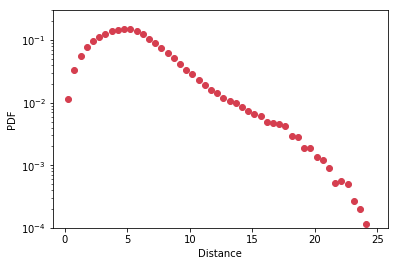
\includegraphics[width=0.9\linewidth]{fig/clark.png}
\caption{The population distribution as a function of distance from a district's center. The vertical axis is logarithmic processed, which represents the exponential decaying of population distribution. Regardless of the finite-sample effect, we fit the middle part of population density's spatial distribution to the exponential distribution with a slope of $-0.95$, which approximately equals to $1-1/\beta.$ This fit has a confidential measurement of $R^2=0.99$.}
\label{fig:clark}
\end{figure}

\section{Spatial coherence}

\section{Relative relationship between urban memory and urban size}

We give a numerical tests for this discussion. 

\section{Phase two: resource restrictions}

\subsection{superior switching} 

Regional development is complex and is affected by differnet determinants in different time. For example, in Hebei province of China, the largest city Shijiazhuang started to develop fast since it is the crossroad of railways. We interpret this as the redistribution of social resource. 

There have been plenty of literations\cite{bowles2019neolithic} that illustrate the interplay between social development and injustice. Social development 



\subsection{urban shrinkage}

The urban development is a sequel of the spatial distribution of existing resource. Thus the preferential attachment is not only performed among people, but also on urban land-use. The concentration of urban resource result in urban shrinkage, indicating that the popular definition of resource distribution, say Gross Democratic Product (GDP), may not be the best indicator of regional furtune, since it is not a perfect indication of a place's future 




% \begin{thebibliography}{99}
%     % \bibitem{David:1970} H.A. David, H.N. Nagaraja, {\it Order statistics}  (John Wiley \& Sons, Inc., 1970).
%     % \bibitem{Massey:1951} F.J. Massey, {\it Journal of the American statistical Association} {\bf 46}, 68-78 (1951).
% \end{thebibliography}
\bibliographystyle{plain}
\bibliography{ref}
    
\end{document}